\newpage
\section{Project management}
Scrum worked well as a project management framework. Combining this with our adaptation of Extreme Programming has led to a very agile and responsive development process. This section will evaluate the team's project management process.

\subsection{Preventive measures}
In order to ensure that the productivity continuously peaked, preventative measures were taken early on in the project. One of these measures were that the team instated a monetary penalty for arriving late to meetings or not delivering work on time. The money accumulated from this was later spent on a team building. The other measure was that one team member was responsible for bringing snacks and making sure the team took regular breaks during the long work sessions on Wednesdays. This arrangement circulated throughout the project. The team believe that both of these measures had a good effect, and that they increased the productivity and mood during work sessions.

\subsection{Working with the customer}
 Initially, there were some problems with the customer not reaching deadlines set in conjunction with the team. This effected the team's research in the early stages of the project. Getting information about the CoSSMic group's research earlier in the project might have changed the course of the product. 

\subsection{Changing roles}
\label{sec:unbalancedWorkload}
In the beginning of the project, the team distributed roles with different areas of responsibility, as described in table~\ref{sec:mainresp}. Almost halfway through the project it became clear that the Scrum master at the time, Per Øyvind, also was the team member with the most experience in Android development. This resulted in a lot of extra work on the Scrum master, while the deputy project leader only had a few responsibilities. The team reviewed the project roles and the workload distribution, which resulted in a change of roles. The team came to the conclusion that Lars Erik, the now former deputy project leader, was best fit to take over the role as Scrum master. After this change, the team's best Android resource could focus entirely on the Android development, and make himself available to help others. The team was satisfied with this decision, and efficiency and productivity increased after the change in roles.

\subsection{Choice of development methods}

The team used Scrum together with XP, described in section~\ref{sec:scrumDevProcess}. Although Scrum is a well known development method, a lot of the team members had different expectations to how the framework would be implemented in the project. This resulted in a lot of excess discussions and was recognized as a risk (8)~\ref{tab:risktable}. The team resolved this issue by consulting the supervisor. Besides this, the team's adaption of Scrum, together with XP, worked great. 

\subsection{Underestimation of workload}
A prevalent risk to any project is the failure to acknowledge the cost of tasks in the project, and the improper allocation of resources that follows such an error. This can also lead to a false sense of what a team can achieve in a given time frame. 

The team experienced this risk(1)~\ref{tab:risktable} to have the biggest negative impact on the work flow. Even though it did not have a detrimental effect on the sprint end result, it was the most occurring risk, which added up to be very time consuming. The main reason for this issue was the lack of experience with many of the tasks, but also that initially the team did not consider who the tasks were assigned to. This turned out to play an important role in the equation. Learning from previous mistakes, the team started looking at previous sprint backlogs to help with the estimation of the tasks.

\subsection{Choice of Scrum tool}
\label{sec:choiceScrumTool}
As the team did not have daily meetings, a good Scrum tool was needed to keep track of progress. Having bad experiences with Scrum tools from previous projects, the team decided to spend some time to research the possible candidates. After Yodiz was chosen, the team were confident that this was the best decision, considering all available options. This still might be true, but using Yodiz nonetheless proved to be somewhat frustrating for the team members. An example of an event that caused a lot of frustration in the early stages of the project is given in the subsequent section. Another example is that the burn down charts that Yodiz generated turned out to be useless for documentation. This led to the team having to do the burn down charts manually. As a matter of fact, a digital Scrum tool is very hard to design in an intuitive fashion. Combined with poor support for simultaneous editing and a lot of down-time for the web-page, the result was a system that caused problems. 

However, Yodiz was the only tool that covered all the requirements set by the team, and despite its flaws, it did its job. Ideally, the team would have liked to have a meeting room with a Scrum board so the use of such an extensive Scrum tool could be avoided altogether. At the end of the project the team started using a Scrum board in the meeting room that was used during the work sessions. The team could have started using this earlier in the project.

\subsubsection{Improper use of Yodiz}
\label{sec:improperScrum}
Despite the team's efforts to get acquainted with Yodiz, a misunderstanding arose, and was not discovered until the end of the second sprint.

The misunderstanding, displayed in figure~\ref{fig:wrongUse}, was that the team
assumed one could add multiple individuals as responsible on a particular task,
while Yodiz' functionality only assigned the time spent to the individual that was assigned as owner of the task.

As a result, it appeared as if only single individuals performed the tasks, even though the entire team in reality was participating. This was also reflected in the burn down charts. 

To sort out this issue, the team went through old meeting reports and time sheets to figure out which members of the team that had actually participated on the particular task. With this information, new tasks for each team member was created.

This issue was unfortunate, but not insurmountable, and not a critical
issue for the overall progress of the project.

\begin{figure}[H]
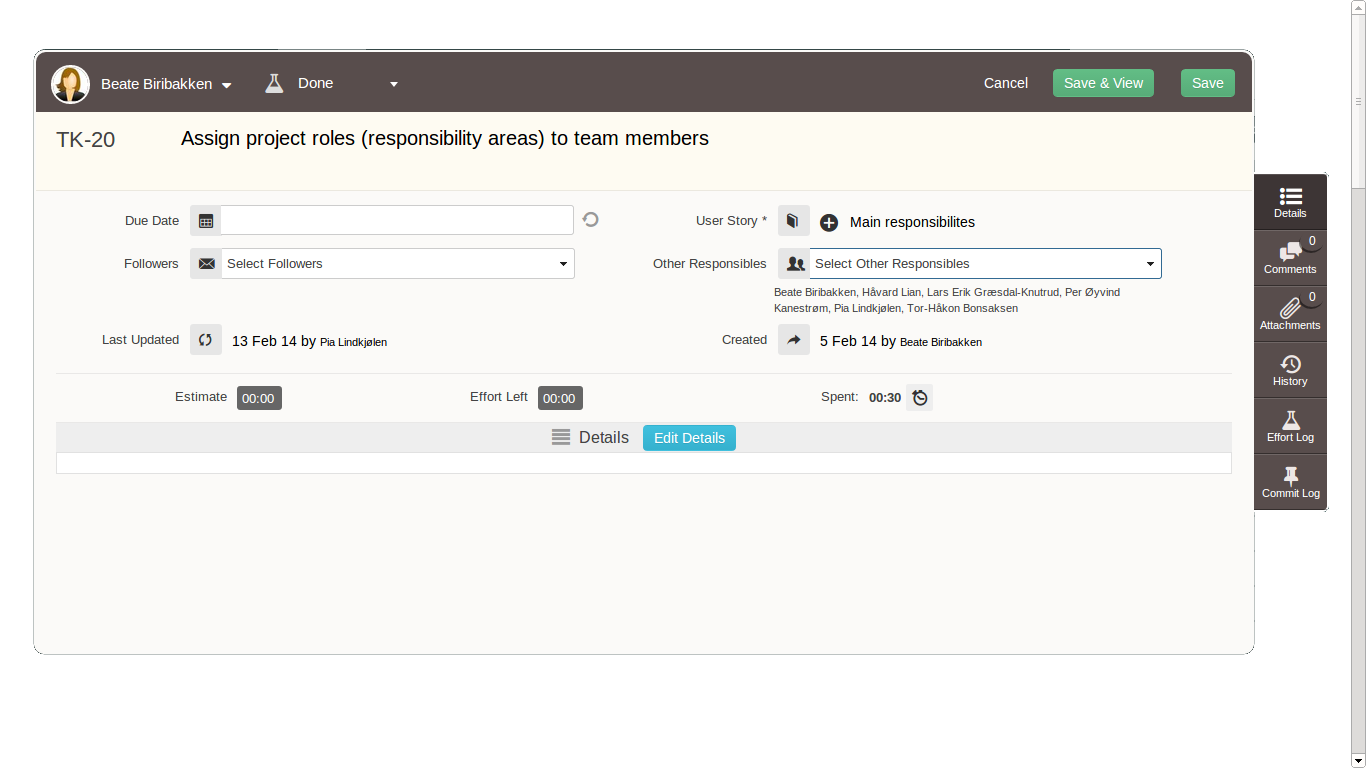
\includegraphics[width=\textwidth, clip, trim=1cm 2cm 4cm 1cm]{ch/retrospect/fig/wrongUse.png}
\caption{Example screenshot to illustrate improper use of Yodiz}
\label{fig:wrongUse}
\end{figure}

